\documentclass{article}
\usepackage[frenchb]{babel}
\usepackage{amsfonts}
\usepackage{amsmath}
\usepackage[T1]{fontenc}
\usepackage[utf8]{inputenc}
\usepackage{amsthm}
\usepackage{graphicx}
\usepackage{tikz}

\usepackage{hyperref}
\hypersetup{                    % parametrage des hyperliens
    colorlinks=true,                % colorise les liens
    breaklinks=true,                % permet les retours à la ligne pour les liens trop longs
    urlcolor= blue,                 % couleur des hyperliens
    linkcolor= blue,                % couleur des liens internes aux documents (index, figures, tableaux, equations,...)
    citecolor= cyan               % couleur des liens vers les references bibliographiques
    }


\title{Géométrie de l'information et apprentissage distribué}
\author{Clément Dell'Aiera, Clément Prévosteau, David Wahiche}
\date{}

\theoremstyle{definition}
\newtheorem{definition}{Définition}
\newtheorem{thm}{Théorème}
\newtheorem{ex}{Exercice}
\newtheorem{lem}{Lemme}
\newtheorem{dem}{Preuve}
\newtheorem{prop}{Proposition}
\newtheorem{cor}{Corollaire}
\newtheorem{conj}{Conjecture}

\newcommand{\Z}{\mathbb Z}
\newcommand{\R}{\mathbb R}
\newcommand{\C}{\mathbb C}
\newcommand{\Hil}{\mathcal H}
\newcommand{\Mn}{\mathcal M _n (\mathbb C)}

\begin{document}
\maketitle

\begin{figure}[h]\centering
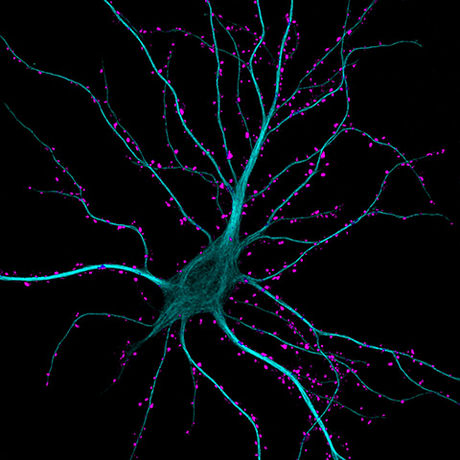
\includegraphics[scale=0.6]{Neurone.jpg}
\caption{Neurone grossi 63 fois, image de Kieran Boyle}
\label{fig:Neurone}
\end{figure}

\newpage
\tableofcontents

\newpage
%%%%%%%%%%%%%%%%%%%%%%%%%%%%%%%%%%%%%%%%%%%%%%%%%%%%%%%%%%%%%%%%%%%%%%%%%%%%%%%%%%%%%%%%%%%
\begin{abstract}
\end{abstract}
%%%%%%%%%%%%%%%%%%%%%%%%%%%%%%%%%%%%%%%%%%%%%%%%%%%%%%%%%%%%%%%%%%%%%%%%%%%%%%%%%%%%%%%%%%%
\section{Réseau de neurones}
Parmi les premières méthodes d'apprentissage figurent celles utilisant des réseaux neuronaux. %Brève explication de ce qu'est un RN ?

Le but de ce travail est d'étudier ce réseau et d'appliquer les méthodes de géométrie de l'information pour peut-être mieux comprendre les raisons de leur efficacité.%Petit topo sur la géometrie de l'info ?
\subsection{Présentation}

Les réseaux de neurones ont initialement été développé comme des algorithmes, initialement dans le domaine de \textit{l'intelligence artificielle}, ce qui en fait naturellement une discipline du \textit{machine learning}. L'idée première était de s'inspirer du fonctionnement du cerveau humain pour créer des algorithmes adaptatifs. Bien que ce rôle fondateur de modèle pour le cerveau humain n'ai pas été un franc succès, les réseaux neuronaux ont donné des modèles statistiques intéressants. Ce changement d'interprétation est reflétée dans le nom de réseau de neurones \textit{artificiels} que certains auteurs utilisent désormais. \\

L'apprentissage est classiquement divisé en plusieurs domaines :
\begin{itemize}
\item apprentissage supervisé : apprendre à prévoir un output lorsque l'on donne un input, divisé en 2 catégories :
\begin{itemize}
\item régression 
\item classification
\end{itemize}
\item Non-supervisé : découvrir une bonne représentation de l'input.
\item Apprentissage par réenforcement : sélection des actions en maximisant le gain.\\
\end{itemize}
Les réseaux de neurones font partie de l'apprentissage supervisé : on se donne une liste d'exemple, le \textit{training set}, et l'on se sert de la différence entre la réponse attendue et la réponse donnée pour corriger l'algorithme.\\

Historiquement, on peut faire remonter l'origine des réseaux de neurones à McCulloch et Pitts en 1943 : ils proposent de modéliser formellement les neurones par des unités traitant un signal d'entrée, renvoyant en sortie un signal binaire correspondant à $1$ si le signal d'entrée dépasse un certain seuil, ce qu'ils nomment un \textit{binary threshold neurons} ou des unités de décisions.\\

Le perceptron constitue la première génération de réseaux neuronaux au sens où on l'entend aujourd'hui, popularisés par Fran Rosenblatt dans les années 60 et dont on trouvera un très bon exposé dans son livre \textit{Principles of Neurodynamics}.\\

Le lecteur pourra aussi trouver dans \textit{Perceptrons} de Minsky et Papert (1969) de quoi satisfaire sa curiosité. Ces deux auteurs sont à l'origine d'un résultat très négatif pour les perceptrons : le thèorème d'invariance sous l'action d'un groupe ("Group invariance theorem"), qui assure que les perceptrons ne peuvent pas apprendre des configurations invariantes sous l'action d'un groupe de transformations. Ce résultat est assez limitant puisqu'il empêche, par exemple, le perceptron d'apprendre des configarations de pixels qui sont invariantes par translations, typiquement ce qu'on aimerait lui faire faire. C'est là que les réseaux multicouches permettront de sauver la mise, comme nous le verrons.\\

Un réseau de neurones peut se formaliser de la façon suivante : plusieurs couches de neurones (que l'on imagine les unes superposées aux autres), chaque couche recevant des signaux de la couche précédentes. Chaque neurone $N_i$ est en fait un opérateur, qui agit sur les signaux d'entrés qu'il reçoit $y_j$ : il leur affecte chacun un poids $w_{ij}$ et ensuite une fonction, signal qu'il transmet à son tour :
\[y_i=f(b+\sum_{i\rightarrow j}w_{ij}y_j)=f(w^T.x)\]
où l'on prend $w$ le vecteur poids associé au neurone $N_i$.\\

Voici une liste non-exhaustive de différents réseaux de neurones, que l'on présente en fonction de leur fonction de réponse :
\begin{itemize}
\item binaire : $y=1_{b+w^Tx>0}$
\item linéaire : $y=b+w^Tx$
\item linéaire rectifié : $y=max(0,b+w^Tx)$
\item sigmoïde : $y=\frac{1}{1+e^{-z}}$
\item binaire stochastique :$\mathbb P(s=1)=\frac{1}{1+e^{-z}}$ L'output est traité comme le paramètre de Poisson.\\
\end{itemize}

Ainsi que plusieurs types d'architectures que l'on peut leur imposer, c'est-à-dire comment les neurones sont reliés entre eux :
\begin{itemize}
\item Une couche ou plusieurs (deep neural networks)
\item Récurrents : des cycles sont possibles.
\item Complets.
\item Toute structure imagnable sur un graphe ! En fait, le modélisateur n'est pas obligé d'adopter une strucutre en couches.\\
\end{itemize}

%%à réaccorder correctement
Ces réseux peuvent se reformuler en termes de modèles statistiques, comme Herbert K.H.Lee l'expose dans \textit{Bayesian Non Parametrics via Neural Networks}. Rappelons qu'un réseau est composé de plusieurs couches : la couche d'entrée, les couches cachées et la couche de sortie. Chaque noeud du réseau applique une fonction $\psi$, en général une sigmoïde, à une combinaison linéaire des signaux d'entrée. Si $y$ est le signal de sortie, $x$ l'entrée, le modèle statistique que représente le réseau à $m$ couches cachées prend souvent la forme :

\[y=\beta_0 \sum_{i=1}^m \beta_i\psi(w_i^T x_i) + \eta_i\]
\[\eta_i \sim \mathcal N(0,\sigma^2)\]

Cet équation montre qu'un réseau neuronal peut s'interpréter comme un modèle de régression non paramétrique sur une base donnée. Par exemple, si 
\[\psi(x)=\frac{1}{1+\exp(-x)}\]
est la fonction logistique, on sait que l'espace engendré par les translatés-échelonnés de cette fonction est tout l'espace des fonctions de carré intégrable.

%Un exemple simple : 2 couches de  neurones.
%\begin{itemize} \item Top $=$ formes connues. \item Bottom $=$intensité des pixels.\end{itemize} Chaque pixel peut voter (pour plusieurs formes) s'il est colorié. \\

Détaillons un peu différents modèles simples de RN.

 \subsection{Neurones binaires et algorithme du "perceptron convergence procedure"}
Ces neurones ont une fonction deréponse de type indicatrice :
\[y=1_{\{w^Tx\geq 0\}}\]

Voici comment entraîner les neurones binaires comme classifiants :\\

\fbox{\begin{minipage}{0.9\textwidth}
\begin{enumerate}
\item Incorporer une composante $1$ en plus au vecteur input, pour incorporer le biais dans les poids.
\item Choisir un exemple d'entraînement. La procédure de choisx doit assurer que tous les exemples seront choisis.
\item Si l'output est correct, ne pas changer les poids. Sinon soustraire l'input du vecteur des poids.
\end{enumerate}
\end{minipage}}\\
\\

On peut interpréter géométriquement cette procédure.\\

L'ensemble des poids est vu comme un $\R$-espace vectoriel de dimension le nombre de poids. Un input définit un hyperplan (son orthogonal), et un vecteur poids donne la bonne réponse par rapport à cet input ssi il est du "bon côté" du plan. Si on a deux inputs, le sous-ensemble des bons poids (qui répondent correctement aux deux inputs) forment alors un cône. On remarque que les bons poids forment un ensemble convexe : le problème est convexe.\\

\begin{dem}%la faire vraiment
On suppose qu'il existe un vecteur $w^*\in C$ qui donne la bonne réponse à tous les exemples.\\
\[|w_{n+1}-w*|^2=|w_n-x|^2=|w_{n+1}|^2+|x|^2+2\langle w_n,x\rangle+|w^*|^2+2\langle w^*,w_n-x\rangle \leq |x|^2\]
\qed
\end{dem}

\subsection{Neurones linéaires ou filtres linéaires}
On appelle neurones linéaires des neurones dont la focntion de réponse est linéaire :
\[y=w^Tx\]

Ici l'algorithme, plutôt que d'approcher de mieux en mieux le poids idéal, va optimiser la distance entre l'ouput et la cible, ce qui est une différence notable par rapport au cas précédent. La procédure des neurones binaires (perceptron) ne peut pas se généraliser à plusieurs couches et nous prévenons le lecteur : leur nom de "perceptron multicouches" utilisé à propos des neurones linéaires est un faux ami ! \\

Voici l'algorithme :\\

\fbox{\begin{minipage}{0.9\textwidth}
Choisir un pas d'apprentissage $\epsilon$.
\begin{enumerate}
\item On entraîne en donnant la cible $t$.
\item Actualiser les poids selon : \[\Delta w_i = \epsilon x_i(t-y)\]
\end{enumerate}
\end{minipage}}\\
\\

On comprend que cet algorithme n'est rien d'autre qu'une descente de gradient. En effet, si on dérive l'erreur quadratique : \[E=\frac{1}{2}\sum_{n\in training}(t^n-y^n)^2\]
on obtient : $\frac{\partial E}{\partial w_j}=-\sum x_i^n(t^n-y^n)$. Cette règle d'actualisation des poids (\textit{batch delta-rule}) modifie les poids proportionnelement à cette dérivée afin de se rapporcher du minimum de la surface d'erreur :
\[\Delta w_i =-\epsilon \frac{\partial E}{\partial w_j}\]


\subsubsection{La surface d'erreur du neurone linéaire}
On se place dans l'espace des poids, augmenté d'une dimension pour l'erreur. On s'intéresse donc au graphe de l'erreur :

\[\mathcal S = \{(w_1,..,w_n,E)\}\]

Dans le cas d'un RN linéaire avec erreur quadratique, c'est un paraboloïde elliptique. L'algorithme précédent effectue une descente le long de ce paraboloïde, perpendiculairement aux lignes de niveau (qui sont des ellipses). Cela explique que l'apprentissage puisse être très lent : si l'ellipse est très aplatie, le gradient peu pointer dans une direction très peu colinéaire au minimum recherché. ( d'où la correction avec le gradient riemanien)

\newpage
\begin{figure}[!h]\centering
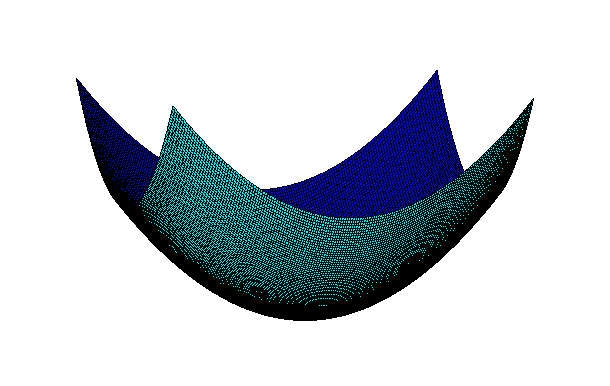
\includegraphics[scale=0.5]{Surfaceerreur.png}
\caption{La forme typique d'une surface d'erreur quadratique.}
\label{fig:Surface}
\end{figure}

\begin{figure}[!h]\centering
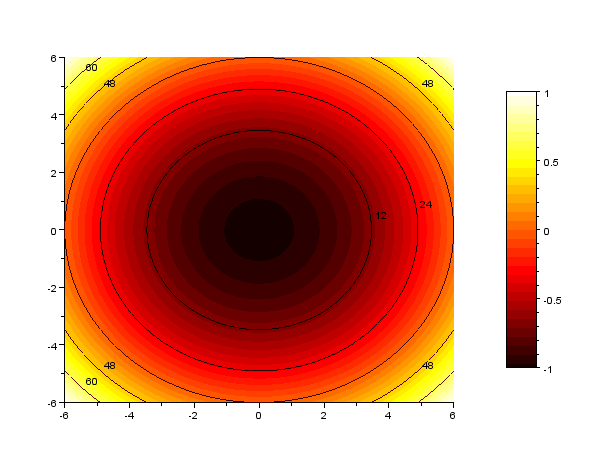
\includegraphics[scale=0.5]{level.png}
\caption{Les lignes de niveau d'une surface d'erreur quadratique sont bien des ellipses. }
\label{fig:level}
\end{figure}

\newpage


\subsubsection{Pourquoi plusieurs couches?}

\noindent Ici considérons le cas particulier du XOR dessiné ci-dessous. $ABCD$ est un carré des les sommets diagonalement opposés sont de même couleur. On cherche à prédire leur couleur. Il y a deux couleurs, ce problème peut donc se rapporter à un problème de prédiction de vecteurs binaires.

\begin{figure}[h!]
\begin{center}
\begin{tikzpicture}\centering
\draw  (-1,-1) grid [step=1cm] (2,2);
\draw (0,0) node[black,below left]{$A$}node[red]{$\bullet$};
\draw (1,1) node[black,above right]{$C$}node[red]{$\bullet$};
\draw (0,1) node[black,above left]{$B$}node[blue]{$\bullet$};
\draw (1,0) node[black,below right]{$D$}node[blue]{$\bullet$};
%\draw[black] (0,0) rectangle (1,1);
\draw[blue,dashed] (-1,1/2)--(2,1/2);
\end{tikzpicture}
\end{center}
\label{XOR}
\caption{Représentation graphique du <<ou exclusif>>.}
\end{figure}


\noindent Dans ce cas-là, une réseau à une seule couche nous donne un classifieur linéaire qui ne permet pas de séparer les points de couleurs différentes. Ainsi en rajoutant une couche intermédiaire, qui permet d'obtenir deux classifieurs linéaires et leur intersection permet de reconnaître le XOR.

\begin{figure}[h!]
\begin{center}
\begin{tikzpicture}\centering
\node[draw,circle] (A)at(0,2) {$X_1$};
\node[draw,circle] (B)at(0,0) {$X_2$};
\node[draw,circle,fill=gray!50] (C)at(3,2) {$H_1$};
\node[draw,circle,fill=gray!50] (D)at(3,0) {$H_2$};
\node[draw,circle,] (E)at(1.5,3) {$1$};
\node[draw,circle,] (F)at(6,1) {output};
\tikzstyle{radial}=[very thick,->,>=stealth];
\draw[->,>=latex](A)--(C)
	node[midway,below]{$W_{1,1}$};
\draw[->] (B)--(C)
	node[pos=0.1,above]{$W_{1,2}$};
\draw[->](A)--(D)
	node[pos=0.25,left]{$W_{2,1}$};
\draw[->](B)--(D)
	node[pos=0.5,below]{$W_{2,2}$};
\draw[->](E)--(C)
	node[pos=0.2,right]{$b_1$};
\draw[->](E)--(D)
	node[pos=0.2,left]{$b_2$};
\draw[->](D)--(F)
	node[midway,below]{$W_2$};
\draw[->](C)--(F)
	node[midway,above]{$W_1$};
\draw[->](E) to[bend left]node[midway,above]{$b_0$}(F);
\end{tikzpicture}
\end{center}
\label{RN2}
\caption{Réseau de neurones à deux couches.}
\end{figure}


\noindent Ainsi pour le premier neurone, on pose $u_1=W_{1,1}x_1+W_{1,2}x_2+b_1$ et $u_2=W_{2,1}x_1+W_{2,2}x_2+b_2$. On effectue la somme logique et on obtient par exemple la séparation de l'espace suivante:
\begin{figure}[h!]
\begin{center}
\begin{tikzpicture}
\draw (0,0) node[black,below left]{$A$}node[red]{$\bullet$};
\draw (1,1) node[black,above right]{$C$}node[red]{$\bullet$};
\draw (0,1) node[black,above left]{$B$}node[blue]{$\bullet$};
\draw (1,0) node[black,below right]{$D$}node[blue]{$\bullet$};
%\draw[black] (0,0) rectangle (1,1);
\draw[blue] (-1,1)--(2,-1);
\draw[red] (0,2)--(2,-1);
\filldraw[fill=gray!20,opacity=0.5] (-1,1)--(2,-1)--(0,2)--cycle;
\end{tikzpicture}
\end{center}
\label{Dessin}
\caption{Séparation non linéaire}
\end{figure}

\noindent La zone grise obtenue correspond à l'intersection des deux séparateurs linéaires. On voit qu'on peut bien reconnaître le xor qui permet bien de séparer les points de couleur différente. Le théorème de l'approximation universelle pour les réseaux neuronaux va plus loin: avec des fonctions d'activation sigmoïdales, on peut approximer pour n'importe quelle constante arbitraire une fonction continue sur un sous-ensemble compact de $\R^n$.


\newpage
\noindent Mathématiquement , cela nous donne:
\begin{thm}
Soit $\phi$ une fonction non constante, bornée et de limites finies en $+$ et $-\infty$ différentes. Soit $X \subseteq \R^m$ et $X$ compact. Alors:

\noindent $\forall f \in \mathcal{C}(X),~\forall \epsilon>0;~\exists n\in \mathbb{N},(a_{i,j})\in\R^n\times\R^m,(b_i)\in \R^n,(w_i)\in\R^n:~~||f-A_n f||<\epsilon$

\noindent avec $(A_n f)(x_1,...,x_m)=\displaystyle\sum_{i=1}^n w_i \phi\left(\displaystyle\sum_{j=1}^m a_{i,j}x_j+b_i\right)$
\end{thm}

\subsubsection{Expériences autour du Xor}

\noindent On souhaite vérifier si on ne surapprend pas les couleurs des points du Xor. Soient $A(-1,1)$, $B(1,-1)$ des points de couleur rouge et $C(-1,-1)$ et $D(1,1)$ de couleur bleue. On bruite aléatoirement ces points de telle sorte à ce que chaque point du tirage associé à un point demeure dans le quart de plan de ce point. On obtient ainsi la figure suivante.

\begin{figure}[!h]\centering
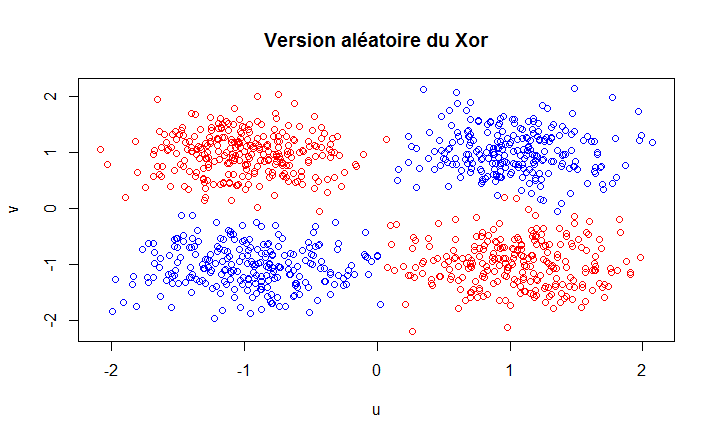
\includegraphics[scale=0.5]{xoralea.png}
\caption{Représentation d'un tirage de xor aléatoire}
\label{fig:xoralea}%le label neurone etait deja pris
\end{figure}

\noindent Une \textbf{SVM}, ou machine à vecteurs de support constituent une généralisation des classifieurs linéaires. Ils ont été développés dans les 1990 à partir des théories de Vladimir Vapnik.

\noindent Ils permettent de traiter des problèmes de discrimination non-linéaire, et de reformuler le problème de classement comme un problème d'optimisation quadratique. Leur fonctionnement repose sur deux idées:
\begin{itemize}
\item la recherche de la \textit{marge maximale}: la marge est la distance entre la frontière (linéaire) de séparation et les échantillons les plus proches qu'on appelle \textit{vecteur supports}. Dans les SVM, on cherche à maximiser la marge
\item le problème principal des SVM si laissés comme tels est qu'ils ne permettent pas de reconnaître des formes non linéairement séparables. L'idée utilisée pour remédier à ce genre de problèmes est d'augmenter potentiellement la dimension de l'espace dans lequel on cherche les hyperplan séparateurs en appliquant par exemple une transformation non-linéaire $\phi$ aux vecteurs d'entrée $x$. Ainsi dans le cas d'un cercle non identifiable en coordonnées cartésiennes, le passage en coordonnées polaires permet de répondre à la question. On appelle ces transformations des \textit{noyaux} qui doivent vérifier certaines conditions et ces techniques sont appelées \textit{kernel trick}.
\end{itemize}

\noindent De manière plus théorique, pour répondre à un problème de discrimination, c'est-à-dire à quelle classe appartient un échantillon, on considère le problème suivant $l=h(x)$ avec $x$ les données d'entrée et $l\in \{-1,1\}$ le label (on se limite ici au cas où il n'y a que deux types). On cherche $h$ de la forme $h(x)=w^Tx+w_0$ avec $w=(w_1,...,w_N)$ un vecteur de poids. Si $h(x)\geq0$, alors $x$ est de classe $1$, $-1$ sinon. L'ensemble $\{x/h(x)=0\}$ est appelé \textit{hyperplan séparateur}.

\noindent Ainsi l'algorithme d'apprentissage supervisé a pour but d'apprendre $h$ à l'aide des données $\{(x_1,l_1),...,(x_p,l_p)\}\subset \R^N\times\{-1,1\}$ avec $(l_i)$ les labels des vecteurs d'entrée, $p$ la taille de la base d'apprentissage et $N$ la dimension des vecteurs d'entrée. Si le problème est linéairement séparable, on a:

$l_k\times \left(w^T x_k+w_0\right)\geq 0$ pour tout $1\leq k \leq p$

\noindent Dans le cas d'un problème linéairement séparable, il existe une infinité d'hyperplans séparateurs. Vapnik a montré (ref à mettre) que la capacité des classes d'hyperplans séparateurs diminue avec l'augmentation de la \textit{marge} définie comme \textbf{la distance des points de l'hyperplan séparateur aux vecteurs} $x_k$. La capacité ou \textit{dimension VC} correspond au \textbf{cardinal du plus grand ensemble séparé par une fonction} $f$. Selon la règle du Rasoir d'Occam,et afin d'éviter une surprédiction des données, les SVM suivent le programme suivant:
arg$\displaystyle\max_{w,w_0}\min_k\{||x-x_k||;x\in \R^N,w^tx+w_0=0\}$.

\noindent Ce qui équivaut à
arg$\displaystyle\max_{w,w_0}\left\lbrace\frac{1}{||w||}\min_k\left[l_k \left(w^T x_k+w_0\right)\right]\right\rbrace$.

\noindent Pour faciliter l'optimisation, on normalise $w,w_0$ de telle sorte à ce que les \textit{vecteurs supports}, qui sont les plus proches de l'hyperplan, satisfassent:
\begin{equation*}
w^Tx_{k}+w_0=\begin{cases}
	-1\\
	1
\end{cases}
\end{equation*}
\\
\noindent Ainsi maximiser la marge revient donc à maximiser $\frac{1}{||w||}$. On s'est ramené au problème
\fbox{\begin{minipage}[c]{0.9\textwidth}
maximiser $\frac{1}{2}||w||^2$ sous les contraintes $l_k\left(w^T x_k+w_0\right)\geq 1$
\end{minipage}}\\ 

\noindent On choisit de maximiser $\frac{1}{2} ||w|||^2$ plutôt que $||w||$ pour des raisons pratiques dans l'écriture du lagrangien. 

\noindent Ce problème se résout à l'aide d'un calcul de Lagrangien dont les conditions permettent notamment de remarquer que l'hyperplan solution ne dépend que du produit scalaire entre le vecteur d'entrée et les vecteurs supports. Par conséquent, on peut modifier le système de coordonnées pour passer d'un espace non linéairement séparable à un espace non linéairement séparable - comme le passage des coordonnées cartésiennes aux coordonnées polaires pour un cerle.

\noindent On en arrive donc au \textit{kernel trick}. Cette fois, on cherche un hyperplan séparateur $h(x)=w^T f(x)+w_0$ qui vérifie $l_k h(x_k)>0$. Cela revient en fait à changer les $x_k$ en $f(x_k)$ avec $f$ une transformation qui peut être non linéaire.

\noindent En suivant le même procédé que précédemment, on se ramène donc au problème d'optimisation suivant:


\fbox{\begin{minipage}[c]{0.9\textwidth}
Maximiser $L(\alpha)=\displaystyle\sum_{k=1}^p\alpha_k-\frac{1}{2}\displaystyle\sum_{i,j} \alpha_i\alpha_j l_i l_j f(x_i)^T f(x_j)$ \\
sous les contraintes $\alpha_i \geq 0$ et $\displaystyle \sum_{k=1}^p\alpha_k l_k=1$
\end{minipage}}\\


\noindent $h$ est alors de la forme

\fbox{\begin{minipage}[c]{0.45\textwidth}
$h(x)=\displaystyle \sum_{k=1}^p\alpha_k^* l_k K(x_k,x)+w_0$\\
avec $K(x_k,x)=f(x_k)^T*f(x)$
\end{minipage}}
\\
\newpage
\begin{figure}[!h]\centering
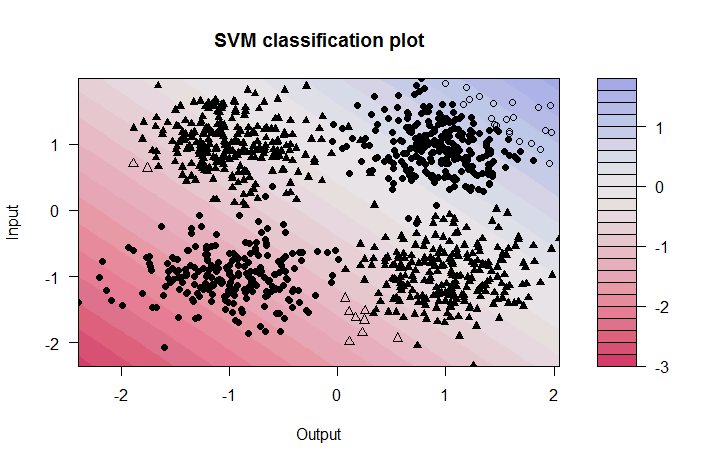
\includegraphics[scale=0.6]{svmlinxor.png}
\caption{Reconnaissance par un svm \textbf{linéaire} du xor}
\label{fig:svmlinxor}
\end{figure}

\noindent On voit sur la figure ci-dessus que les points noircis correspondent aux erreurs obtenues avec un SVM linéaire. Les résultats obtenus sont mauvais car les points du XOR ne sont pas linéairement séparables.

\newpage

\noindent En revanche, en ayant recours au kernel trick, avec un noyau polynomial de degré $2$, les résultats sont bien meilleurs. Ils sont de la forme $K(x,y)=(x^T y+c)^2$ où $x$ et $y$ sont les vecteur d'entrée et $c\geq 0$ une constante.

\begin{figure}[!h]\centering
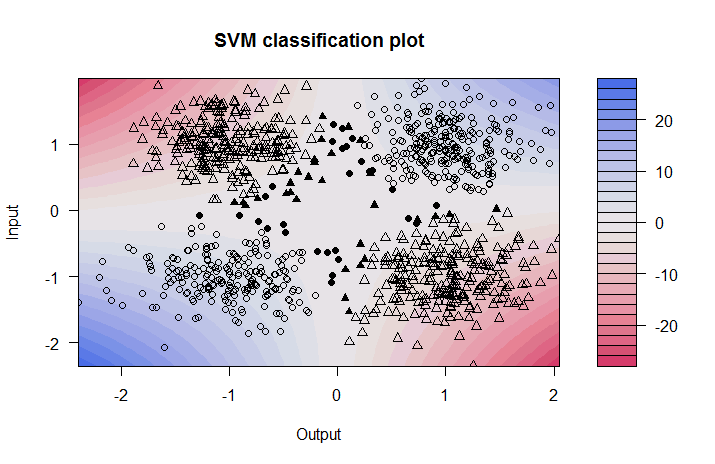
\includegraphics[scale=0.6]{svmxorplydot.png}
\caption{Reconnaissance par un svm  avec un noyau \textbf{de degré $2$} du xor}
\label{fig:svmpolydot}
\end{figure}

\newpage

\begin{figure}[!h]\centering
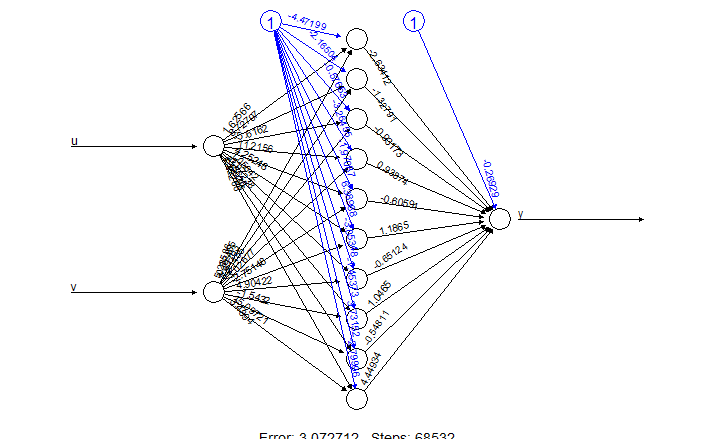
\includegraphics[scale=0.6]{nnxor.png}
\caption{Reconnaissance par un réseau neuronal du xor}
\label{fig:nnxor}
\end{figure}

%je n'ai pas trop d'idées encore sur la manière dont il faudrait commenter ce schéma...

\newpage

\subsection{Neurones logistiques}

On va généraliser la procédure précédente aux réseau de neurones logistiques, ceux qui ont une fonction de réponse du type : 
\[z=b+w^Tx\]
\[y=\frac{1}{1+e^{-z}}\]
On remarque que l'image de la fonction logistique est l'intervalle $(0;1)$, ce qui nous permettra d'interpréter sa valeur comme la probabilité de l'output sachant l'input, dans le cas de réseaux de neurones stochastiques. 
\[\frac{\partial y}{\partial w_i}=x_i y(1-y)\]
\[\frac{\partial E}{\partial w_j}=-\sum_{n}x_i^n(1-y^n)y^n(t^n-y^n)\]

\subsection{Algorithme de rétropropagation}

Maintenant que l'on sait modifier les poids pour une seule couche, on va donner un moyen de modifier les poids dans le cas de couches cachées. Cette généralisation n'est pas innocente : les réseaux sans couche cachée ne sont pas très adaptables, au sens où leur modélisation est beaucoup plus limitée que celle des réseaux multicouches. L'idée de la rétropropagation est de remonter les dérivées des erreurs par rapport au output récursivement à travers les couches cachées, de la couche des ouptu à celle des input. On suppose bien sûr que l'erreur est dérivable, rendant cet algorithme inutile pour un réseau binaire par exemple.\\

Soit donc un neurone $N_j$ situé dans une couche cachée. Il reçoit un input total 
\[z_j=\sum_{i\rightarrow j} w_{ij}y_i.\]
On cherche alors à calculer l'erreur $\frac{\partial E}{\partial y_i}$ pour tous les neurones qui lui sont connectés dans la couche précédente, \textit{ie} les neurones $N_i$ tels que $i\rightarrow j$. Mais une simple application de la règle de la chaîne donne une expression simple pour ce terme :

\[\frac{\partial E}{\partial z_j}=\frac{\partial y_j}{\partial z_j}\frac{\partial E}{\partial y_j}=y_j(1-y_j)\frac{\partial E}{\partial y_j}\]
\[\frac{\partial E}{\partial y_i}=\sum_j\frac{\partial z_j}{\partial y_i}\frac{\partial E}{\partial z_j}=\sum_j w_{ij}\frac{\partial E}{\partial z_j}\]
Donc :\\

\fbox{\begin{minipage}[c]{0.45\textwidth}
\[\frac{\partial E}{\partial y_i}=\sum_j w_{ij}y_j(1-y_j)\frac{\partial E}{\partial y_j}\]
\end{minipage}}\\
\\
On peut alors calculer la variation de l'erreur en fonction d'une variation des poids :
\[\frac{\partial E}{\partial w_{ij}}=\frac{\partial z_j}{\partial w_{ij}}\frac{\partial E}{\partial z_j}=y_i\frac{\partial E}{\partial z_j}.\]

Bien que cette procédure nous guide pour adapter les poids, plusieurs questions se posent en pratique, par exemple : à quelle fréquence doit on mettre à jour nos poids ? Comment choisir la vitesse d'apprentissage ? On peut adapter les poids à chaque exemple (\textit{online}), après tout le stock d'exemple (\textit{full batch learning}), ou bien encore après un petit nombre (\textit{mini batch}).\\

%%%%%%%%%%%%%%%%%%%%%%%%%%%%%%%%%%%%%%%%%%%%%%%%%%%%%%%%
\subsection{}
Softmax : forcer les outputs à former une probabilité
Problème de l'erreur quadratique : mauvais avec une fonction logistique , les dérivées tendent à "plateau out" lorsque l'output $y$ ets proche de $0$ ou $1$ : 
\[\frac{dE}{dz}=(t-y)y(1-y)\]
Une erreur plus convenable est la cross entropy function :
\[E=-t\log(y)-(1-t)\log(1-y)\] 
car alors \[\frac{dE}{dz}=y-t\]
Pour un groupe de neurones $N_i$ qui recoivent en entrée $z_i$ appelée \textit{logit}, l'output est donné par 
\[y_i=\frac{e^{z_i}}{\sum_{j\in group} e^{z_j}}\]
\[\frac{dy_i}{dz_i}=y_i(1-y_i)\]
Corss entropy : la bonne fonction de coût \[C=-\sum_j t_j \log(y_j)\quad t_j \ \text{target value}\]

\subsection{Point de vue géométrique}

Nous présentons dans cette section les idées de différents articles d'Amari, ainsi que de son livre \textit{Methods of information Geometry}.\\

Comme nous l'avons remarqué, les réseaux de neurones peuvent s'interpréter comme un modèle statistique à réponse non linéaire : $y=f(x,w)$, et en supposant que les données suivent la densité $q(x)$ et qu'on a la densité conditionnelle $p(y|x,w)$, l'ensemble des données $(x,y)$ suivent la loi :

\[q(x)p(y|x,w)\]

Les modèles de perceptrons que nous présenterons ensuite sont considérés pa Amari comme des points d'une variété qu'il appelle \textit{Neuromanifold}, où les coordonnées sont les $w$ et la métrique est donnée par l'information de Fisher.\\

\subsection{Machines de Boltzmann}

\subsubsection{Introduction}

\noindent Un autre exemple fortement lié aux réseaux de neurones est celui de la \textbf{machine de Boltzmann}, qui est un réseau totalement connecté de $n$ neurones stochastiques. Chacun des neurones $N_i$ possède un état $x_i$ qui est $0$ ou $1$, qu'il communique en \textit{output} aux autres neurones. L'algorithme d'apprentissage est très lent de manière générale pour les réseaux multicouches mais est rapide dans le cadre des "restricted Boltzmann machines" (que l'on notera RBM) qui ne comporte qu'une seule couche de détecteurs de caractéristiques.


\noindent Les machines de Boltzmann sont utilisées pour la résolution de deux types de problèmes. Pour un problème de recherche, les poids (même typologie que pour les réseaux neuronaux)sont fixés et sont utilisés dans une fonction de coûts. Ce type de machine permet alors d'échantillonner des vecteurs à valeurs binaires de sorte pour lesquels la fonction de coût est faible.

\noindent Dans le cas d'un problème d'apprentissage, la machine de Boltzmann dispose en entrée de vecteurs de données binaires et apprend à générer ce type de vecteurs avec une forte probabilité. Pour ce faire,les poids doivent être modifiés de sorte à ce que par rapport à d'autres vecteurs binaires les données d'entrées prennent de faibles valeurs de la fonction de coût. Afin de résoudre ce type de problèmes, la machine met à jour les poids et chaque mise à jour nécessite nécessite la résolution de beaucoup de problèmes de recherche différents.

\subsubsection{Dynamique stochastique d'une machine de Boltzmann}

\noindent Chaque neurone calcule la quantité
\[u_i=\sum_{j \neq i} w_{ij}x_j-h_i\]
en fonction des signaux qu'il reçoit. Le poids $w_{i,j}$, appelé poids de la connexion synaptique, mesure l'influence du neurone $N_j$ sur le neurone $N_i$, et $h_i$ est appelé le seuil de $N_i$. On suppose que la matrice des poids $W= [w_{i,j}]$ est symétrique à diagonale nulle.\\
A chaque étape, chaque neurone $N_i$ détermine s'il sera dans l'état excité $1$ ou dans l'état de repos $0$ selon la probabilité :

\[\mathbb P(x_i=1)=\frac{e^{u_i}}{1+e^{u_i}}\]

L'état de la machine de Boltzmann est représenté par le vecteur $x=(x_1,...,x_n)$, qui suit une chaîne de Markov sur l'espace de tous les états possibles, espaces à $2^n$ points. Cet chaîne admet comme loi stationnaire :
\[p^{W,h}(x)=\frac{1}{Z}\exp\{-E(x)\}\]
\[\text{avec} \quad E(x)=-\frac{1}{2}x^TWx +h^Tx\]
\[\text{et} \quad Z=\sum_x \exp\{-E(x)\}\]

On peut prendre le point de vue géométrique en se représentant la machine de Boltzmann comme une système qui se comporte selon la loi stationnaire $p^{W,h}(x)$, donc comme un point de coordonnées $(W,h)$ dans la variété de toutes les machines de Boltzmann. ( Encore un exemple de famille exponentielle. )

\noindent Afin de déteminer dans lequel la ième unité se trouve, dans un premier temps on calcule l'input total noté $z_i$ qui est la somme du biais associé à cette unité $b_i$ et des poids sur les connections provenant des autres unités \textbf{activées}:
\begin{align*}
z_i=b_i+\sum_{j}s_j w_{i,j}
\end{align*}

\noindent avec $s_j$ l'état de l'unité $j$ et $w_{i,j}$ le poids associé à la connection entre $i$ et $j$.

\noindent L'unité $i$ passe en position "on" avec la probabilité donnée par la fonction logistique:
\begin{align*}
\mathbb{P}(s_i=1)=\frac{1}{1+\exp(-z_i)}
\end{align*}

\noindent Si les unités sont mises à jour séquentiellement dans un ordre quelconque, le réseau tend vers sa distribution stationnaire dans laquelle la probabilité d'un vecteur d'état est déterminé uniquement par son "énergie" par rapport à toutes les énergies de tous les autres vecteur d'état binaire.

\begin{align*}
\mathbb{P}(\vec{v})=\frac{\exp(-E(\vec{v}))}{\sum_{\vec{u}} \exp(-E(\vec{u}))}\\
\textit{avec E définie par}\\
E(\vec{v})=-\sum_i s_i^{v} b_i-\sum_{i < j} s_i^{v} s_j^{v} w_{i,j}
\end{align*}

\noindent où $s_i^v$ est l'état de l'unité donnée par le vecteur d'état $\vec{v}$.

\subsubsection{Learning dans les machines de Boltzmann}

\textbf{Sans couches cachées}

\noindent Etant donné un ensemble de vecteurs d'état d'entraînement, apprendre consiste à trouver les poids et biais (paramètres) qui permettent d'obtenir une distribution stationnaire pour laquelle les vecteurs d'état ont une forte probabilité.Par différentiation dans les équations ci-dessus, on obtient:
\begin{align*}
\left\langle\frac{\partial \log \mathbb{P}(\vec{v})}{\partial w_{i,j}}\right\rangle_{data}=-\frac{\partial E(-\vec{v})}{\partial w_{i,j}}-\frac{\partial\sum_{\vec{u}} \exp(-E(\vec{u}))}{\partial w_{i,j}}\\
\left\langle\frac{\partial \log \mathbb{P}(\vec{v})}{\partial w_{i,j}}\right\rangle_{data}=\left\langle s_is_j\right\rangle_{data}-\left\langle s_is_j\right\rangle_{model}
\end{align*}

\noindent avec $\langle.\rangle_{data}$ est une espérance associée à la distribution des datas et $\langle.\rangle_{model}$ est l'espérance obtenue lorsque la machine de Boltzmann a une distribution stationnaire. La remontée de gradient s'effectue à partir de:
$w_{i,j}=w_{i,j}+\epsilon \left\langle s_is_j\right\rangle_{data}-\left\langle s_is_j\right\rangle_{model}$

\noindent De même, $b_i=b_i+\epsilon \left\langle s_i\right\rangle_{data}-\left\langle s_i\right\rangle_{model}$.

\textbf{Avec couches cachées}

\noindent On dit qu'il y a des couches cachées si les états de certaines unités ne sont pas déterminés par les données visibles. L'intérêt de ce type de couches est qu'elles permettent à la machine de Boltzmann de modéliser des distributions sur les données visibles qui ne pourraient pas être modélisées par des interactions par paires entre les unités visibles. Toutefois la règle d'apprentissage demeure inchangée. Dans ce cas,
$\langle s_i s_j\rangle_{data}$  est la moyenne sur tous les vecteurs d'entrées de $s_i s_j$ lorsque le vecteur d'entrée est fixé et qu'on actualise les couches cachées jusqu'à l'équilibre.

\subsection{Restricted Boltzmann machines}

\subsubsection{Introduction}

\noindent Une RBM est constituée d'une couche visible et d'une couche cachée. Il n'y a pas de connections entre les unités visibles ni entre les unités cachées. Par conséquent, les unités de la couche cachées sont conditionnellement indépendantes étant donné un vecteur d'entrée "visible". Ainsi échantillonner à partir de $\langle s_i s_j\rangle_{data}$ s'obtient en une étape parallélisée. On a néanmoins toujours besoin de plusieurs itérations d'actualisation des poids de la couche cachée et de la couche visible pour échantillonner à paritr $\langle s_i s_j\rangle_{model}$. Toutefois on peut remplacer $\langle s_i s_j\rangle_{model}$ par $\langle s_i s_j\rangle_{reconstruction}$ que l'on obtient de la manière suivante:
\begin{itemize}
\item Un vecteur visible en entrée et on met à jour toutes les unités de la couche cachée
\item Mettre à jour les unités de la couche visible pour obtenir une "reconstruction"
\item Mettre à jour à nouveau toutes les unités de la couche cachée.
\end{itemize}

\noindent Cette procédure d'apprentissage approxime la descente de gradient et on l'appelle "constrastive divergence".

\subsubsection{Deep Learning à l'aide de RBM}


\noindent Après apprentissage dans la couche cachée, les vecteurs d'activation de cette couche peuvent être considérés à leur tour comme des données d'entraînement pour une nouvelle machine de Boltzmann et ce de manière répétée. C'est la partie d'apprentissage non-supervisé.

\noindent Les probabilités conditionnelles peuvent donc s'écrire, avec $\vec{v}$ le vecteur des données visibles et $\vec{h}$ celui des données de la couche cachée:
\begin{align*}
\mathbb{P}(\vec{v}|\vec{h})=\prod_{i=1}^m \mathbb{P}(v_i|\vec{h})\\
\mathbb{P}(\vec{h}|\vec{v})=\prod_{j=1}^n \mathbb{P}(h_j|\vec{v})
\end{align*}

\noindent On peut écrire:
\begin{align*}
\mathbb{P}(h_j=1|\vec{v})=\sigma\left(b_j+\sum_{i=1}^m w_{i,j} v_i\right)\\
\mathbb{P}(v_i=1|\vec{h})=\sigma\left(b_j+\sum_{j=1}^n w_{i,j} h_j\right)\\
\end{align*}

\noindent avec $\sigma$ la fonction d'activation logistique.

\noindent Ainsi les RBM sont entraînées à maximiser le produit des probabilités associés à un ensemble d'entraînement $V$ et détermine $argmax_W \prod_{\vec{v}\in V}\mathbb{P}(\vec{v})$ ou de manière équivalente $argmax_W \mathbb{E}\left[\sum_{\vec{v}\in V} \log\left(\mathbb{P}(\vec{v})\right)\right]$

\subsubsection{Précisions sur l'algorithme de Contrastive divergence (noté CD-1)}

\noindent Revenons sur l'algorithme décrit brièvement plus haut:
\begin{itemize}
\item On prend un échantillon d'entraînement $\vec{v}$, on calcule les probabilités des unités cachées et on échantillonne un vecteur d'activation caché $h$ de cette distributions
\item On calcule le produit dyadique de $v$ et $h$ que l'on appellera le gradient positif
\item De $h$, on échantillonne une reconstruction $v'$ d'unités visibles puis on rééchantillonne $h'$ de $v'$
\item On calcule le produit dyadique de $v'$ et $h'$ que l'on appellera le gradient négatif
\item On actualise les poids en leur ajoutant le gradient positif moins le gradient négatif multiplié par un taux d'apprentissage $\epsilon$ : $\Delta w_{i,j}=\epsilon (vh^T-v'h'^T)$. On effectue la même chose pour les biais $a$ et $b$.
\end{itemize}

\noindent Ainsi si l'on note $\textbf{v}^0$ le vecteur initial et qu'on répète la procédure initiale en échantillonnant selon l'algorithme de Gibbs, on obtient:
\begin{align*}
\frac{\partial \log p(\textbf{v}^0)}{\partial w_{i,j}}=\langle v_i^0 h_j^0\rangle-\langle v_i^{\infty} h_j^{\infty}\rangle
\end{align*}

\subsection{Deep Belief Networks}

\noindent Mes Deep Belief Nets sont des modèles générant une loi jointe à partir d'observations et des labels associés composés de plusieurs couches de variables qualitatives stochastiques. De manière classique, ces variables qualitatives prennent des valeurs binaires et on les appelle \textit{unités cachées}. Le deux couches du dessus ont des connections symétriques non-dirigées entre elles et constituent la mémoire associative : on peut associer un vecteur binaire d'entrée à un autre vecteur qui lui associe sa valeur. Les couches du dessous ont des connections dirigées haut-bas provenant de la couche du dessus. Les états des unités de la couche la plus en bas représentent les vecteurs de données.

\noindent Les deux propriétés les plus importants des Deep Belief Nets sont:
\begin{itemize}
\item il existe un procédé d'apprentissage efficace d'apprentissage des poids haut-bas qui donnent la dépendance des unités d'une couche en fonction des unités de la couche supérieure.
\item Après apprentissage, toutes les unités cachées peuvent être inférés en un seul passage haut-bas qui commence avec un vecteur de données observé dans la couche la plus basse et qui utilise les poids calculés pendant l'apprentissage dans la direction inverse.
\end{itemize}

\noindent Les nets sont appris couche par couche en traitant les variables d'une couches, lorsqu'elles sont inférées par les données d'entrée à leur tour comme des données d'entraînement pour la couche suivante.

\noindent On peut améliorer la précision dans le cas discriminant en ajoutant une couche finale de variables qui représentent les valeurs de sortie attendues et utilisant l'algorithme de retropropagation des erreurs des dérivées.

\noindent Une idée au coeur des deep belief network est que les poids $W$ appris par une RBM servent à définir à la fois $p(v|h,W)$ et la distribution a priori des vecteurs cachés $p(h|W)$. Par conséquent, la probabilité d'un vecteur \textit{visible} $v$ s'écrit comme :

$p(v)=\displaystyle \sum_h p(h|W)p(v|h,W)$.

\noindent Après apprentissage des poids, on conserve $p(v|h,W)$ mais on remplace $p(h|W)$ par un meilleur modèle qui est l'agrégation des distributions a posteriori, c'est-à-dire la distribution non factorielle obtenue en effectuant la moyenne des distributions factorielles a posteriori issues par chacun des vecteurs de données.

\noindent Comme on a pu l'observer précédemment, l'initialisation des poids revêt une importance fondamentale dans la vitesse de convergence des algorithmes de descente de gradient. C'est pourquoi dans le cas de modèles complexes comme la reconnaissance d'images on entraîne dans un premier temps le modèle de manière non supervisée afin d'initialiser les poids.

\begin{tikzpicture}\centering
\node[draw] (H0)at(0,0){\Large $H_0$};
\node[draw] (V0)at(0,-2){\Large $V_0$};
\node[draw] (V1)at(0,2){\Large $V_1$};
\node[draw] (H1)at(0,4){\Large $H_1$};
\node[draw] (P)at(0,6){};
\draw [<->] (H1.north)--(P.south)node[midway,right]{$W_3$};
\draw [->] (V1.40)--(H1.-40)node[midway,right]{$W_2^T$};
\draw [->] (H0.40)--(V1.-40)node[midway,right]{$W_1^T$};
\draw [->] (V0.40)--(H0.-40)node[midway,right]{$W_0^T$};
\draw [<-] (V1.100)--(H1.-100)node[midway,left]{$W_2$};
\draw [->] (H0.100)--(V1.-100)node[midway,left]{$W_1$};
\draw [->] (V0.100)--(H0.-100)node[midway,left]{$W_0$};
\end{tikzpicture}

\noindent On peut imaginer recourir aux RBM dans un premier temps . On utilise l'algorithme suivant:
\begin{enumerate}
\item Apprendre $W_0$ en supposant que toutes les matrices de poids sont liées : ici l'actualisation des poids se déroulent comme expliquée dans les RBM
\item Détermination de $W_0$ et on utilise $W_0^T$ pour déterminer les distributions a posteriori factorielles es variables de la première couche cachées $H_0$
\item En considérant toutes les matrices de poids des couches supérieures comme liées sauf $W_0$, apprentissage d'un modèle RBM des couches supérieures à partir des données générées par $W_0^T$ et leur transformation sur les données initiales.
\end{enumerate}

\noindent Les relations haut-bas correspondent aux poids de reconnaissance et ceux bas-haut aux poids de génération. Apprendre les matrices des poids couche par couche est efficace mais pas optimal. Une fois que les matrices de poids des couches supérieures ont été calculés, ni les poids, ni le procédé d'inférence de base sont optimaux dans les couches inférieures. On considère alors les matrices de poids de reconnaissance comme indépendantes de celles de génération, en revanche on conserve le fait que le postérieurs de chaque couche peut être approximé par une distribution factorielle selon laquelle les variables d'une même couche sont indépendantes conditionnellement aux variables de la couche du dessous.  Cependant si on effectue une procédure \textit{up-pass}, à savoir l'utilisation des poids de reconnaissance dans un \textit{bottom-up pass} qui tire sotchastiquement l'état des couches cachées. Les poids des connections dirigées sont alors ajustés en utilisant la règle d'optimisation du maximum de vraisemblance utilisée dans l'algorithme de contrastive divergence. Les poids des couches sans connections dirigées sont calculées en fittant la RBM du haut sur les distribution a posteriori de l'avant =-dernière couche. la \textit{down-pass} part d'un état de la mémoire associative et utilise les connections haut-bas de génération pour activer stochastiquement les couches inférieures séquentiellement. Au cours de cette procédure, seuls les poids bas-haut de reconnaissance sont actualisés.

\subsection{Multilayer Neural Network}

On se donne un réseau de neurones spécifié par un paramètres $w\in \R^n$, qui représente les poids modifiables des connexions entre les synapses. En entrée du réseau, le signal $x$, qui suit une loi de probabilité inconnue $q(x)$, est traité, et le réseau calcule une sortie $f(x,w)$. \\

Le but est d'entraîner les neurones : on est en apprentissage supervisé. Lorsque l'on donne l'entrée $x$ au réseau,on peut donc lui spécifier quelle sortie $y$ lui correspond. La discussion qui suit permettra de comprendre comment nous pouvons élaborer un algorithme qui, par itération, améliore les poids jusqu'à atteindre un poids possiblement optimal $w^*$.\\

Soit $L$ une fonction de perte, typiquement : 
\[L(x,y,w)  = ||y-f(x,w)||^2.\] 
En considérant un modèle statistique où le but est une version bruité du signal de sortie, avec un bruit normal centré, ie :
\[y=f(x,w)+\eta\]
\[\text{avec} \quad \eta \sim \mathcal N (0,I_n)\]
la densité du couple $(x,y)$ prend la forme :
\[cq(x)\exp\{-\frac{1}{2}||y-f(x,w)||^2\}.\]

Face à une série d'exemples $(x_1,y_1),...,(x_N,y_N)$, l'algorithme naturel de descente est donné par :
\[w_{n+1}=w_n - \epsilon_n \nabla l(x_n,y_n,w_n), \]
où $l$ est le $\log$ de la densité du couple $(x,y)$, et $\epsilon_n$ est le pas d'apprentissage. Cet algorithme nous fait nous déplacer sur l'espace des réseau de neurones paramétrés pas $w$. Dans Amari\textit{1985}, on peut donner une structure de variété riemannienne à cet espace, structure dont la métrique est donnée par :
\[g_{ij}(w)=\mathbb E[\partial_i p(x,y,w)\partial_j p(x,y,w)].\]

\subsection{Cas du perceptron}

On peut obtenir une forme explicite pour le percptron multicouche.
Ici, la fonction signal est donnée par : \[f(u)=\frac{1-e^{-u}}{1+e^{-u}}\], et $y=f(w.x)+\eta,\quad \eta \sim \mathcal N (0, \sigma^2)$.\\

La densité conditionnelle de $y$ sachant $x$ est alors :
\[p(y|x,w) = \frac{1}{\sqrt{2\pi}\sigma}\exp\{-\frac{1}{2\sigma2}||y-f(x,w)||^2\},\]
ce qui, combiné à l'hypothèse $q(x)$ gaussienne, donne une densité jointe :

\[p(x,y,w) = q(x)p(y|x,w) \]

Le théorème suivant, dont la preuve se trouve dans  \textit{Natural Gradient worksefficiently in learning}, donne explicitement la forme de la métrique de Fisher dans le cas du perceptron multicouches, sous nos hypothèses.

\begin{thm}{(Amari)}
La métrique de Fisher vaut : 

\[G(w)=|w|^2 c_1(w)I_n + (c_2(w)-c_1(w))w\otimes w\]
où :
\[c_1(w)=\frac{1}{4\sqrt{2\pi}\sigma^2|w|^2}\int (f^2(wt)-1)^2\exp(-\frac{1}{2}t^2)dt\]
\[c_2(w)=\frac{1}{4\sqrt{2\pi}\sigma^2|w|^2}\int (f^2(wt)-1)^2t^2\exp(-\frac{1}{2}t^2)dt\]

La matrice inverse est : 
\[G^{-1}(w)=\frac{1}{|w|^2 c_1(w)}I_n+\frac{1}{|w|^4}(\frac{1}{c_2(w)}-\frac{1}{c_1(w)})w\otimes w\]
\end{thm}
 
Nous pouvons alors donner une formule explicite pour l'algorithme de gradient naturel :
\[w_{n+1}=w_n + \epsilon_n(y_n-f(w_n.x_n))f'(w_n.x_n)
	\{ \frac{1}{|w_n|^2c_1(w_n)}x_n+\frac{1}{|w_n|^4}( \frac{1}{c_2(w)}-\frac{1}{c_1(w)}) w_n.x_n w_n\}\]

En guise de remarque finale pour cette partie, mentionnons que cette méthode se généralise facilement ( bien qu'avec plus de calculs ) au cas d'un perceptron multicouche à sortie linéaire, possédant $m$ couches. 
La relation \textit{input-output} s'écrit ici :
\[y=\sum_{i=1}^m v_i f(w_i.x)+\eta\]
\[\eta \sim \mathcal N(0,I_n)\]

Le calcul de $G^{-1}$ est plus facile que dans le cas classique ( comparez l'inversion d'une matrice $(n+1)\times m$ à celle d'une matrice $2 \times (m+1)$ ), et Amari et G. Yang ont effectué des études sur cette méthode : elle pourrait éviter l'effet plateau que les méthodes classiques peinent tant à eviter.

%%%%%%%%%%%%%%%%%%%%%%%%%%%%%%%%%%%%%%%%%%%%%%%%%%%%%%%%%%%%%%%%%%%%%%%%%%%%%%%%%%%%%%%%%
%%%%%%%%%%%%%%%%%%%%%%%%%%%%%%%%%%%%%%%%%%%%%%%%%%%%%%%%%%%%%%%%%%%%%%%%%%%%%%%%%%%%%%%%%
%%%%%%%%%%%%%%%%%%%%%%%%%%%%%%%%%%%%%%%%%%%%%%%%%%%%%%%%%%%%%%%%%%%%%%%%%%%%%%%%%%%%%%%%%
\section{Point de vue géométrique en statistique}
%%%%
%%%%

\subsection{Géométrie de l'information}

La géométrie de l'information propose d'utiliser les méthodes de la géométrie différentielle en statistique afin d'optimiser les algorithmes. Pour le lecteur apeuré par les gros mots mathématiques, qu'il se rassure : il n'est pas question ici d'étudier les propriétés géométriques fines des objets statistiques, mais plutôt d'appliquer des outils à peine plus sophistiqués que ceux d'un cours de calcul différentiel classique dans une optique d'optimisation.\\

 L'idée première est de donner une structure de variété différentielle au modèle statistique étudié : si $\mathcal S = \{p_\theta\}_\theta$ est notre honnête famille paramétrique de lois de probabilité, on peut voir $\theta \in \Theta$ comme une coordonnées, ou, pour parler le langage des géomètres, l'application : \[p_\theta \mapsto \theta\] fournit une carte locale. Petite remarque : cette application n'est définie que si le modèle est identifiable. On supposera d'ailleurs que le modèle a toutes les propriétés que l'on voudrait.\\

La deuxième étape est de donner une structure de variété riemannienne au modèle $\mathcal S$. Sans rentrer dans les détails, l'important est de savoir que l'on peut définir une métrique grâce à la log-vraisemblance $l$ du modèle par :
\[g_{ij} (\theta) = \mathbb E_\theta[\partial_i l(X,\theta) \partial_j l(X,\theta)]\]
En pratique, cela signifie que l'on peut mesurer des distances et des angles sur l'espace tangent à $\mathcal S$ : 
\[\forall w_1,w_2 \in T_\theta \mathcal S, \langle w_1 , w_2 \rangle = w_1^T G w_2\] où $G(\theta)=(g_{i,j}(\theta))_{ij}$.\\

Donnons un exemple important : celui des familles exponentielles. Le modèle est donné par :
\[\mathcal{E}xp(C,F,\psi) = \{p(x,\theta)=\exp[C(x)+\sum_{i=1}^n \theta^i F_i(x) -\psi(\theta)] \quad :\quad  \theta \in \R^n\}\]
où $F=(F_1,...,F_n)$ est une famille linéairement indépendante de fonctions $C^\infty$. Un simple calcul donne :
\[\partial_i \partial_j l(x,\theta) =-\partial_i \partial_j \psi(\theta)\]
Donc :
\[g_{ij}(\theta) =\mathbb E[\partial_i l(x,\theta)\partial_j l(x,\theta)]=-\mathbb E[\partial_i\partial_j l(x,\theta)]=\partial_i \partial_j \psi(\theta)\]
La matrice $G$ est donc la hessienne de $\psi$ et on a calculé la métrique riemannienne :
\[ds^2= \sum_{i,j} \partial_i \partial_j \psi \ dx^i dx^j\]

\subsection{Algorithme de descente de gradient naturel}

\noindent Amari décrit dans ses différents articles ~\cite{Amari1994} ~\cite{Amari1998} une méthode de descente de gradient adapté au cadre riemannien : on va corriger le pas par un facteur qui va se révéler être l'inverse de la matrice de Fisher. %idéeintuitive avec les ellipses, peut-être une illustration ?

\begin{figure}[h!]
\begin{tikzpicture}
\draw plot[domain=0:2*pi]
	({5*cos(\x r)},{3*sin(\x r)});	
\draw (-5,0)--(5,0);
\draw (0,0)node[below]{$O$}node{$\bullet$};
\draw (-4,0)node[below]{$F_1$}node{$\bullet$};
\draw (4,0)node[below]{$F_2$}node{$\bullet$};
\draw [dashed] plot[domain=-1:5]
	(\x,-0.26*\x+3.27);
\draw [dashed] plot[domain=0.5:2.25]
	(\x,3.82*\x-4.89);
\draw (2,2.75)node[above right]{$A$}node[red]{$\bullet$};
\draw [<-,blue] plot[domain=1.5:2]
	(\x,3.82*\x-4.89);
\draw [->,red] (2,2.75)--(1,1.375);
\draw (1.8,2.802)--(1.86,3)--(2.052,2.95);
\end{tikzpicture}
\label{ellipse}
\caption{En bleu, le gradient euclidien, et en rouge le gradient corrigé. En un point où l'ellipse est très courbée, le gradient riemannien donne une meilleure direction de descente.}
\end{figure}

\noindent Soit $\mathcal{S}$ une variété de $\R^n$. On se donne une fonction de perte $L : \mathcal S \rightarrow \R$ que l'on évalue en $w$, et on veut minimiser $L(w+dw)$ où la norme $|dw|=\epsilon$ est fixée. 
%Néanmoins dans le cas où on peut associer à $\mathcal{S}$ un système de coordonnées orthonormales, on retombe sur la norme classique 
% pas de sens : on peut toujours le faire
Si la norme est fixe pour chaque point et est donnée par la somme des carrés des coordonnées, on retrouve la formule usuelle :
$||dw||^2=\displaystyle \sum_{i=1}^n (dw_i)^2$. La formalisation précédente permet de considérer des espaces plus généraux en permettant à la métrique de varier de façon lisse tout en restant localement euclidienne. En effet, la métrique riemannienne est simplement la donnée d'une matrice symmétrique définie positive $(g_{ij}(p))_{i,j}$ pour chaque point $p$ de la variété $\mathcal{S}$. 
%Dans le cas où on ne peut associer \textbf{localement} à $\mathcal{S}$ un système de coordonnées orthonormées, on pose alors: (idem)
La norme d'un vecteur tangent à la variété $dw$ est alors donnée par :
\[||dw||^2=\displaystyle \sum_{i,j} g_{i,j}(w) dw_i dw_j.\]

 La matrice $G=(g_{i,j})$ est appelée \textit{tenseur métrique riemannien } et l'espace $\mathcal{S}$ est alors un espace \textit{Riemannien}. La descente de gradient habituelle $x \leftarrow x-\eta \nabla f$ est  trouve la direction de la plus grande pente dans le cadre euclidien. Le théorème suivant montre comment adapter cet algortihme au cadre riemannien, c'est-à-dire avec une métrique qui varie. Sur la figure \ref{ellipse}, on aperçoit la différence entre gradient habituel et riemanien. Typiquement, on veut ici minimiser une fonction dont les lignes de niveau sont des ellipses assez aplatie, et donc de diriger vers son centre. Or la métrique donnée par la hessienne de la fonction prend en compte la courbure, alors qu'une descente de gradient euclidienne diverge fortement. Cet exemple sera mis en pratique lors de la section $2$ où l'on étudiera des surfaces d'errerus de réseaux de neurones.\\


\begin{thm}
La direction optimale de descente $dw^*$ est donnée par :
\[dw^*= -\hat{\nabla}L(w)=-G^{-1}(w) \nabla L(w)\]
\end{thm}

\begin{dem} Posons $dw= \epsilon a $, le problème de minimisation devient alors :
\[\min L(w+\epsilon a) \quad s.c. \quad |a|^2=\sum_{i,j} g_{ij}(w)a_i a_j=1\]

Mais $L(w+\epsilon a) - L(w)-\epsilon (\nabla L(w))^T a $ est un petit o de $\epsilon$ et minimiser $(\nabla L(w))^T a$ sous la contrainte $a^T G a = 1$ est simple avec les conditions de Lagrange qui donnent :
\[\frac{\partial}{\partial a_j}((\nabla L(w))^T a - \lambda a^T G a )=0\]
Finalement : $\nabla L(w) = 2\lambda Ga$ et donc 
\[a=\frac{1}{2\lambda}G^{-1}\nabla L(w)\] \qed
\end{dem}

L'algorithme de pas d'apprentissage $\epsilon_n$ qui en découle est décrit par la formule de récurrence suivante :
\[w_{n+1}=w_n -\epsilon_n \hat{\nabla} L(w_n)\] 

\subsection{Métriques invariantes}

Le cadre riemannien permet en apprentissage statistique une meilleure compréhension des algorithmes. Par exemple, celui de descente de gradient habituel peut être adapté comme on l'a vu avec le théorème précédent. Finalement, au prix d'une complexité calculatoire un peu plus grande, l'espace des paramètres d'un modèle peut être vu comme un véritable espace géométrique sur lequel on peut se <<déplacer>>. Se pose le problème du choix de la métrique. Comme le souligne Ollivier dans son article ~\cite{Ollivier}, il est préférable que la métrique ne dépende que du résultat attendu de l'algorithme et non des choix du modélisateur tels que le système de coordonnées (les valeurs accordées aux paramètres). L'on pourrait choisir par exemple de multiplier arbitrairement la métrique par $2$. Et le modèle ne devrait pas réagir à un tel changement. ollivier appelle les métriques qui remplissent un tel cahier des charges des \textit{métriques invariantes}.\\

On note $x\in \mathcal D$ une entrée d'un algorithme paramétré par $\theta \in \mathcal S$, et $w(x)\in \R^d$ la sortie correspondante. On va munir l'espace des paramètres d'une structure de variété riemannienne $(\mathcal S, G)$. Un changement $d\theta$ dans les paramètres induit un changement $dw(x)$ dans la réponse de l'algorithme. On peut alors considérer la norme euclidienne de ce changment $|dwx)|$ et définir la norme d'une variation de paramètre comme l'espérance sur les données $|d\theta|_{nat}^2=E_{x\in \mathcal D}|dw(x)|^2$. Dans le cas d'un réseau de neurones à plusieurs couches, notées $k\in \text{units}$, on définit :
\begin{definition}[Métrique naturelle]
La métrique naturelle est donnée par :
\[|d\theta|_{u,nat}^2=\sum_{k\in\text{units}} |d\theta_k|_{nat}^2.\]
\end{definition}

A aucun moment dans la définition précédente n'est fait mention de paramètres autres que la norme sur l'espace des sorties de l'algortihme : la métrique ne dépend que de ce que fait l'algorithme. Nous renvoyons à l'article d'Ollivier ~\cite{Ollivier} pour une preuve.
\begin{prop}
La métrique naturelle est invariante.
\end{prop}


\subsection{Application à la reconnaissance de caractères manuscrits}

Les algortihmes d'apprentissages sont souvent testés sur la base MNIST disponible à \url{http://yann.lecun.com/exdb/mnist/}. Cette base contient $70 000$ images de chiffres tracés à la main, $60 000$ étant un échantillon d'entraînement, le reste est destiné au test. \\

Le code du projet est entièrement disponible à la page web : \url{https://github.com/cdellaie/GT}.\\

Il consiste en des définitions de classes \textit{python} qui permettent d'implémenter des réseaux de neurones, en laissant le choix des paramètres du modèle à l'expérimentateur. (fonctions d'activations, nombre de neurones, nombre de couches,...) Le code est ensuite testé directement sur la base MNIST.

%A COMPL2TER 

%\subsection{Rappel sur les ondelettes}
%Les ondelettes forment des bases hilbertiennes de $L^2(\R)$ en partant d'une fonction $\phi$, appelée fonction mère, que l'on translate-échelonne ensuite : 
%\[\{2^{j/2}\phi(2^j . -k)\}_{k\in \Z, j \in \Z}.\]
%Par exemple la fonction mère $\phi(u)=1_{0<u<\frac{1}{2}}-1_{\frac{1}{2}<u<1}$ donne la base de Haar, très utilisée en traitement d'image. Voici quelques une de ces fonctions :
%\begin{figure}[h]\centering
%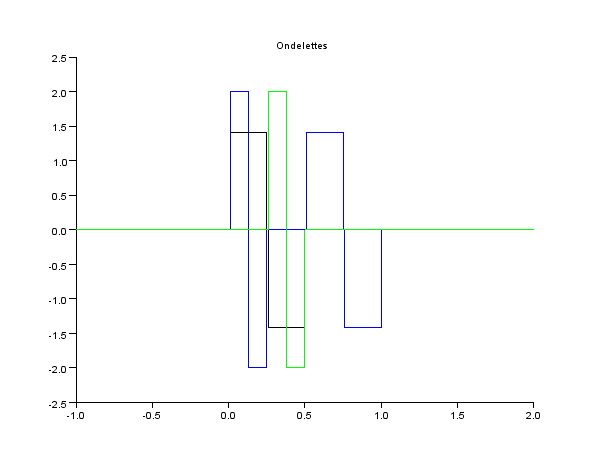
\includegraphics[scale=0.4]{Ondelettes.png}
%\caption{Ondelettes tracées avec Scilab}
%\label{fig:Ondelettes}
%\end{figure}
%\subsection{Description de l'algorithme}
%On entraîne le réseau de neurones avec des images de lettres manuscrites et de la lettre correspondante. Les images sont représentées par un vecteur $N$ dimensionnel, dont les coordonnées sont les $N$ premiers coefficients sur la base d'ondelette.
%\section{Deep Learning vs Support Vector Machine}

%Première Deep Learning architecture : Neocognitron.\\
%Idée : entraîner une couche à la foisen la tratiant comme une machine de Boltzmann restreinte (RBM), et ensuite appliquer un algorithme de Backpropagation.\\
%Rôle de Yan Lecun : première utilisation de l'algorithme de Backpropagation. Disponible depuis les années 70s,cet algorithme était considéré comme trop lent en pratique : problème du vanishing gradient.\\
%\textbf{Algo $em$ et $EM$ ?}

%%%%%%%%%%%%%%%%%%%%%%%%%%%%%%%%%%%%%%%%%%%%%%%%%%%%%%%%%%%%%%%%%%%%%%%%%%%%%%%%%%%%%%%%%%%
\section{Appendice}

\subsection{Géométrie différentielle}


\bibliographystyle{plain}
\bibliography{biblio} 
\nocite{*}

\end{document} 





